\documentclass[11pt,a4paper]{article}

% ---------------------------------------------------------------------------
% Pacotes
% ---------------------------------------------------------------------------
\usepackage[utf8]{inputenc}
\usepackage[T1]{fontenc}
\usepackage[brazilian]{babel}
\usepackage{amsmath,amssymb}
\usepackage{graphicx}
\usepackage{tikz}
\usetikzlibrary{arrows.meta,calc,angles,quotes}
\usepackage{siunitx}
\usepackage{booktabs}
\usepackage{subcaption}
\usepackage{float}
\usepackage[margin=2.5cm]{geometry}
\usepackage{hyperref}
\hypersetup{colorlinks=true,linkcolor=blue!60!black,urlcolor=blue!60!black,citecolor=blue!60!black}

% Caminho das figuras geradas pela simulação (../outputs).
\graphicspath{{../outputs/}}

\title{\textbf{Cinemática Diferencial e Simulação de Robôs Móveis}\\[2pt]
\large Tração Diferencial e Direção de Ackermann}
\author{Guilherme Arthur Allebrandt Schünemann}
\date{}

\begin{document}
\maketitle

% ===========================================================================
\section{Fundamentação Teórica e Dedução Matemática}
% ===========================================================================

A postura (\emph{pose}) de um robô móvel no plano é descrita por
\begin{equation}
  \mathbf{q} = \begin{bmatrix} x \\ y \\ \theta \end{bmatrix},
\end{equation}
onde $(x,y)$ é a posição de um ponto de referência do chassi no
referencial global e $\theta$ é a orientação medida a partir do eixo $X$,
positiva no sentido anti-horário. O objetivo da modelagem cinemática é
relacionar as \emph{entradas de controle} (velocidades das rodas ou
velocidade linear/angular e esterçamento) com as derivadas temporais da
postura $(\dot{x},\dot{y},\dot{\theta})$.

\paragraph{Hipóteses (restrições físicas).} As deduções partem de duas
hipóteses padrão para veículos com rodas em movimento planar:
\begin{enumerate}
  \item \textbf{Rolamento puro (não escorregamento longitudinal):} cada
  roda rola sem deslizar, de modo que a velocidade do ponto de contato ao
  longo do plano da roda vale $v_{\text{roda}} = r\,\omega_{\text{roda}}$,
  com $r$ o raio da roda.
  \item \textbf{Não escorregamento lateral (restrição não-holonômica):} não
  há velocidade na direção do eixo da roda; a roda só se move na direção em
  que aponta. Para o corpo, isso implica que a velocidade lateral do ponto
  de referência é nula:
  \begin{equation}
    -\dot{x}\sin\theta + \dot{y}\cos\theta = 0.
    \label{eq:nonholo}
  \end{equation}
\end{enumerate}
A hipótese de \emph{não capotamento} garante que o movimento permanece no
plano ($z$ constante, sem rotações de rolagem/arfagem), justificando o uso
de um modelo puramente planar de 3 graus de liberdade de postura.

A restrição~\eqref{eq:nonholo} é equivalente a afirmar que o vetor
velocidade do corpo é sempre colinear com a direção de apontamento
$(\cos\theta,\sin\theta)$. Definindo a velocidade linear escalar
$v$ ao longo dessa direção,
\begin{equation}
  \dot{x} = v\cos\theta, \qquad \dot{y} = v\sin\theta,
  \label{eq:body-vel}
\end{equation}
o que satisfaz~\eqref{eq:nonholo} identicamente. As duas subseções a seguir
determinam $v$ e $\dot\theta$ para cada modelo.

% ---------------------------------------------------------------------------
\subsection{Robô com Tração Diferencial}
% ---------------------------------------------------------------------------

\begin{figure}[H]
  \centering
  \resizebox{0.62\textwidth}{!}{% ---------------------------------------------------------------------------
% Geometria do robô de tração diferencial.
%   - chassi alongado, com as rodas motrizes no eixo traseiro (sobre C) e a
%     roda boba (castor) passiva na dianteira, o que dá estabilidade sem
%     alterar a cinemática;
%   - bitola b entre as rodas motrizes; velocidades das rodas v_r, v_l;
%   - referencial do corpo (x_r, y_r) na origem C e ângulo theta em relação
%     ao referencial global.
% ---------------------------------------------------------------------------
\begin{tikzpicture}[>=stealth, scale=1.9]
  % eixo global
  \draw[->, gray] (-0.6,0) -- (3.7,0) node[right]{$X$};
  \draw[->, gray] (0,-0.6) -- (0,2.5) node[above]{$Y$};

  % corpo do robô, orientado por theta; C = ponto médio do eixo traseiro
  \def\thetaval{22}
  \coordinate (C) at (1.4,1.0);
  \begin{scope}[shift={(C)}, rotate=\thetaval]
    % chassi alongado (rodas atrás, roda boba na frente)
    \draw[thick, fill=blue!8] (-0.3,-0.5) rectangle (1.25,0.5);
    % rodas motrizes traseiras (eixo comum passando por C, em x=0)
    \draw[line width=4pt] (-0.18,0.5)  -- (0.18,0.5);   % roda esquerda (+y)
    \draw[line width=4pt] (-0.18,-0.5) -- (0.18,-0.5);  % roda direita (-y)
    % roda boba (castor) dianteira
    \draw[fill=gray!40] (0.98,0) circle (0.09);
    \node[font=\scriptsize] at (0.98,0.26) {roda boba};
    % velocidades das rodas (para frente, ao longo de x_r)
    \draw[->, thick, green!60!black] (0,0.5)  -- (0.65,0.5)  node[above]{$v_l$};
    \draw[->, thick, green!60!black] (0,-0.5) -- (0.65,-0.5) node[below]{$v_r$};
    % bitola b entre as rodas motrizes
    \draw[<->] (-0.28,-0.5) -- (-0.28,0.5) node[midway, left]{$b$};
    % eixos do corpo a partir de C
    \draw[->, thick, red] (0,0) -- (0.78,0) node[above]{$x_r$};
    \draw[->, thick, red] (0,0) -- (0,0.85) node[left]{$y_r$};
    % ponto de referência (meio do eixo traseiro)
    \fill (0,0) circle (1.3pt) node[below left]{$C$};
  \end{scope}

  % ângulo theta entre a horizontal (paralela a X) por C e o eixo x_r
  \draw[dashed, gray] (C) -- ++(1.15,0);
  \draw[->] (C) ++(0.85,0) arc (0:\thetaval:0.85);
  \node at ($(C)+(1.02,0.2)$) {$\theta$};
\end{tikzpicture}
}
  \caption{Geometria do robô de tração diferencial: rodas motrizes separadas
  pela bitola $b$, roda boba (castor) de apoio, velocidades das rodas $v_r$ e
  $v_l$, referencial do corpo $(x_r,y_r)$ e orientação $\theta$.}
  \label{fig:diffdrive-geo}
\end{figure}

O robô possui duas rodas independentes montadas sobre um eixo comum,
separadas pela bitola $b$, e (tipicamente) uma roda-castor livre para
estabilidade. Sejam $\omega_r$ e $\omega_l$ as velocidades angulares das
rodas direita e esquerda. Pelo rolamento puro, as velocidades lineares dos
centros das rodas são
\begin{equation}
  v_r = r\,\omega_r, \qquad v_l = r\,\omega_l.
\end{equation}

Como o corpo é rígido, ambas as rodas compartilham a mesma velocidade
angular $\dot\theta$ em torno do \emph{Centro Instantâneo de Rotação} (ICR),
que se situa sobre o prolongamento do eixo comum das rodas
(Figura~\ref{fig:icr}). Se $R$ é a distância do ICR ao ponto médio do eixo
(ponto de referência $C$), então as rodas descrevem arcos de raios
$R+\tfrac{b}{2}$ e $R-\tfrac{b}{2}$:
\begin{equation}
  v_r = \dot\theta\left(R + \tfrac{b}{2}\right), \qquad
  v_l = \dot\theta\left(R - \tfrac{b}{2}\right).
  \label{eq:dd-arcs}
\end{equation}

A velocidade linear do ponto de referência é a média das velocidades das
rodas, e a velocidade angular vem da diferença. Somando e subtraindo as
equações~\eqref{eq:dd-arcs}:
\begin{align}
  v &\equiv \dot\theta R = \frac{v_r + v_l}{2}
     = \frac{r(\omega_r + \omega_l)}{2}, \label{eq:dd-v}\\
  \dot\theta &= \frac{v_r - v_l}{b}
     = \frac{r(\omega_r - \omega_l)}{b}. \label{eq:dd-w}
\end{align}

Substituindo~\eqref{eq:dd-v} em~\eqref{eq:body-vel} e reunindo com
\eqref{eq:dd-w}, obtém-se o \textbf{modelo cinemático direto do uniciclo}:
\begin{equation}
  \boxed{\;
  \begin{bmatrix}\dot{x}\\[2pt]\dot{y}\\[2pt]\dot{\theta}\end{bmatrix}
  =
  \begin{bmatrix}\cos\theta & 0\\[2pt]\sin\theta & 0\\[2pt]0 & 1\end{bmatrix}
  \begin{bmatrix} v \\ \omega \end{bmatrix},
  \qquad
  \begin{aligned}
    v &= \tfrac{r}{2}(\omega_r+\omega_l),\\
    \omega &= \tfrac{r}{b}(\omega_r-\omega_l).
  \end{aligned}
  \;}
  \label{eq:diffdrive}
\end{equation}

\begin{figure}[H]
  \centering
  \resizebox{0.5\textwidth}{!}{% ---------------------------------------------------------------------------
% Centro Instantâneo de Rotação (ICR) comum.
% Ilustra a restrição de rolamento sem escorregamento: a velocidade de cada
% roda é perpendicular ao raio que a liga ao ICR, de modo que todo o corpo
% gira com velocidade angular theta_dot = v / R em torno do ICR.
% ---------------------------------------------------------------------------
\begin{tikzpicture}[>=stealth, scale=1.2]
  \coordinate (O) at (0,0);
  \fill (O) circle (1.5pt) node[below left]{ICR};

  \def\R{3.0}
  \coordinate (C) at (\R,0);

  % arco de trajetória
  \draw[dashed, gray] (O) circle (\R);
  \draw[->, thick, blue] (\R-0.02,0) arc (0:55:\R);

  % raio R
  \draw[<->] (O) -- (C) node[midway, below]{$R$};

  % robô no ponto C
  \fill (C) circle (1.5pt) node[below right]{$C$};
  % velocidade linear v perpendicular ao raio (tangente)
  \draw[->, thick, red] (C) -- ++(0,1.1) node[right]{$v$};
  % velocidade angular
  \draw[->, thick] (O) ++(35:0.8) arc (35:70:0.8);
  \node at (52:1.15) {$\dot{\theta}=v/R$};
\end{tikzpicture}
}
  \caption{Centro Instantâneo de Rotação: a velocidade $v$ é tangente ao arco
  e $\dot\theta = v/R$.}
  \label{fig:icr}
\end{figure}

\paragraph{Cinemática inversa.} Dado um comando $(v,\omega)$, as
velocidades das rodas necessárias são obtidas invertendo
\eqref{eq:dd-v}--\eqref{eq:dd-w}:
\begin{equation}
  \omega_r = \frac{2v + \omega b}{2r}, \qquad
  \omega_l = \frac{2v - \omega b}{2r}.
  \label{eq:dd-inv}
\end{equation}
Casos particulares: $\omega=0 \Rightarrow \omega_r=\omega_l$ (linha reta);
$v=0,\ \omega\neq 0 \Rightarrow \omega_r=-\omega_l$ (giro puro em torno de
$C$, $R=0$).

% ---------------------------------------------------------------------------
\subsection{Robô com Cinemática de Ackermann}
% ---------------------------------------------------------------------------

\begin{figure}[H]
  \centering
  \resizebox{0.72\textwidth}{!}{% ---------------------------------------------------------------------------
% Geometria da direção de Ackermann.
%   - distância entre eixos L, bitola d;
%   - rodas traseiras fixas, rodas dianteiras esterçadas (interna/externa);
%   - centro instantâneo de rotação (ICR) e raio R do eixo traseiro;
%   - ângulo phi do modelo bicicleta (roda dianteira virtual central).
% ---------------------------------------------------------------------------
\begin{tikzpicture}[>=stealth, scale=1.1]
  % ICR
  \coordinate (O) at (0,0);
  \fill (O) circle (1.5pt) node[left]{ICR};

  % eixo traseiro (a uma distância R do ICR)
  \def\R{3.2}
  \def\L{2.2}
  \def\d{1.4}
  \coordinate (RL) at (\R,0);            % roda traseira esquerda (interna)
  \coordinate (RR) at (\R+\d,0);         % roda traseira direita (externa)
  \coordinate (RC) at (\R+0.5*\d,0);     % centro eixo traseiro
  \coordinate (FC) at (\R+0.5*\d,\L);    % centro eixo dianteiro

  % chassi
  \draw[thick, fill=blue!6] (RL) -- (RR) -- ($(RR)+(0,\L)$) -- ($(RL)+(0,\L)$) -- cycle;

  % rodas traseiras (fixas)
  \draw[line width=4pt] ($(RL)+(0,-0.25)$) -- ($(RL)+(0,0.25)$);
  \draw[line width=4pt] ($(RR)+(0,-0.25)$) -- ($(RR)+(0,0.25)$);

  % raios do ICR até cada roda dianteira
  \draw[dashed, gray] (O) -- ($(RL)+(0,\L)$);
  \draw[dashed, gray] (O) -- ($(RR)+(0,\L)$);
  \draw[dashed] (O) -- (RC);
  \draw[dashed] (O) -- (FC);

  % rodas dianteiras esterçadas (perpendiculares ao raio)
  \draw[line width=4pt, red]  ($(RL)+(0,\L)$) ++(-28:-0.25) -- ++(-28:0.5);  % interna
  \draw[line width=4pt, red]  ($(RR)+(0,\L)$) ++(-20:-0.25) -- ++(-20:0.5);  % externa

  % rótulos de dimensões
  \draw[<->] ($(RL)+(-0.4,0)$) -- ($(RL)+(-0.4,\L)$) node[midway,left]{$L$};
  \draw[<->] (RL) ++(0,-0.6) -- ($(RR)+(0,-0.6)$) node[midway,below]{$d$};
  \draw[<->] (O) ++(0,0.15) -- ($(RC)+(0,0.15)$) node[midway,above]{$R$};

  % angulos
  \node[red] at ($(RL)+(0.55,\L+0.35)$) {$\phi_i$};
  \node[red] at ($(RR)+(0.55,\L+0.35)$) {$\phi_o$};
\end{tikzpicture}
}
  \caption{Geometria de Ackermann: distância entre eixos $L$, bitola $d$,
  ângulos das rodas interna ($\phi_i$) e externa ($\phi_o$) convergindo para
  um ICR comum, e raio $R$ do eixo traseiro.}
  \label{fig:ackermann-geo}
\end{figure}

No veículo tipo automóvel as rodas traseiras são fixas e a esterçamento é
feito pelas rodas dianteiras. A condição geométrica de Ackermann exige que
todas as rodas rolem sem escorregar em torno de um \emph{ICR comum}, situado
sobre o prolongamento do eixo traseiro (Figura~\ref{fig:ackermann-geo}).
Isso impõe que as rodas dianteiras interna e externa tenham \emph{ângulos de
esterçamento distintos}.

\paragraph{Restrição geométrica das duas rodas dianteiras.}
Seja $R$ o raio de curvatura do centro do eixo traseiro, $L$ a distância
entre eixos e $d$ a bitola dianteira. A roda interna está a uma distância
horizontal $R-\tfrac{d}{2}$ do ICR e a externa a $R+\tfrac{d}{2}$. Como
cada roda deve ser tangente ao seu arco (perpendicular ao raio):
\begin{equation}
  \tan\phi_i = \frac{L}{R - \tfrac{d}{2}}, \qquad
  \tan\phi_o = \frac{L}{R + \tfrac{d}{2}}.
  \label{eq:ack-inner-outer}
\end{equation}
Como $R-\tfrac{d}{2} < R+\tfrac{d}{2}$, tem-se $\phi_i > \phi_o$: a roda
interna à curva esterça mais que a externa. Essa é precisamente a
\emph{condição de Ackermann}, que evita o escorregamento lateral dos pneus.
Eliminando $R$ entre as duas relações obtém-se a forma clássica
$\cot\phi_o - \cot\phi_i = d/L$.

\paragraph{Modelo bicicleta (redução).}
Para as equações de estado é conveniente condensar as duas rodas dianteiras
em uma única roda virtual central, com ângulo de esterçamento $\phi$
equivalente, alinhada ao centro do eixo dianteiro. Sua restrição geométrica
é
\begin{equation}
  \tan\phi = \frac{L}{R} \quad\Longrightarrow\quad R = \frac{L}{\tan\phi}.
  \label{eq:ack-radius}
\end{equation}
Tomando como ponto de referência o centro do eixo traseiro, sua velocidade
linear $v$ é tangente à trajetória, satisfazendo~\eqref{eq:body-vel}. A
velocidade angular do corpo é $\dot\theta = v/R$; substituindo
\eqref{eq:ack-radius}:
\begin{equation}
  \dot\theta = \frac{v}{R} = \frac{v\tan\phi}{L}.
  \label{eq:ack-w}
\end{equation}

Reunindo, obtém-se o \textbf{modelo cinemático direto de Ackermann
(bicicleta)}:
\begin{equation}
  \boxed{\;
  \begin{bmatrix}\dot{x}\\[2pt]\dot{y}\\[2pt]\dot{\theta}\end{bmatrix}
  =
  \begin{bmatrix}
    v\cos\theta\\[2pt]
    v\sin\theta\\[2pt]
    \dfrac{v}{L}\tan\phi
  \end{bmatrix},
  \qquad R = \frac{L}{\tan\phi}.
  \;}
  \label{eq:ackermann}
\end{equation}
Esta é a forma apresentada na documentação da MathWorks para o modelo de
bicicleta/Ackermann. Note a analogia com
\eqref{eq:diffdrive}: o papel de $\omega$ é assumido por $\tfrac{v}{L}\tan\phi$,
com a diferença crucial de que existe um raio mínimo de curvatura
$R_{\min}=L/\tan\phi_{\max}$ (o esterçamento é limitado), ao passo que o
robô diferencial pode girar no próprio eixo ($R=0$).

\paragraph{Comparação dos modelos.}
\begin{table}[H]
  \centering
  \begin{tabular}{lll}
    \toprule
    & \textbf{Tração diferencial} & \textbf{Ackermann (bicicleta)} \\
    \midrule
    Entradas & $(v,\omega)$ ou $(\omega_r,\omega_l)$ & $(v,\phi)$ \\
    $\dot\theta$ & $\omega = \frac{r}{b}(\omega_r-\omega_l)$ & $\frac{v}{L}\tan\phi$ \\
    Raio mínimo & $0$ (giro no eixo) & $L/\tan\phi_{\max} > 0$ \\
    Restrição & não-holonômica & não-holonômica \\
    \bottomrule
  \end{tabular}
  \caption{Síntese dos dois modelos cinemáticos.}
\end{table}

% ===========================================================================
\section{Simulação da Cinemática Inversa (Comandos de Movimentação)}
% ===========================================================================

A \emph{cinemática inversa} traduz um comportamento desejado em comandos de
entrada. Para o robô diferencial usamos~\eqref{eq:dd-inv} para converter
$(v,\omega)$ em $(\omega_r,\omega_l)$; para o Ackermann, o comando é
diretamente $(v,\phi)$. Cada cenário é definido por um comando constante por
partes aplicado durante $T=\SI{8}{s}$ (implementado em
\texttt{src/robotica/scenarios.py}):

\begin{table}[H]
  \centering
  \begin{tabular}{lll}
    \toprule
    \textbf{Cenário} & \textbf{Diferencial} $(v,\omega)$ & \textbf{Ackermann} $(v,\phi)$ \\
    \midrule
    Frente          & $(+0{,}5,\ 0)$      & $(+0{,}5,\ 0)$ \\
    Ré              & $(-0{,}5,\ 0)$      & $(-0{,}5,\ 0)$ \\
    Curva esquerda  & $(+0{,}5,\ +0{,}6)$ & $(+0{,}5,\ +25^\circ)$ \\
    Curva direita   & $(+0{,}5,\ -0{,}6)$ & $(+0{,}5,\ -25^\circ)$ \\
    \bottomrule
  \end{tabular}
  \caption{Comandos de entrada por cenário (unidades SI: \si{m/s}, \si{rad/s}, graus).}
\end{table}

\paragraph{Resultados.} As Figuras~\ref{fig:dd-traj} e~\ref{fig:ack-traj}
mostram as trajetórias no plano $(X,Y)$; as figuras de estado
correspondentes (não todas reproduzidas aqui por concisão) registram a
evolução de $x(t)$, $y(t)$ e $\theta(t)$ e encontram-se em
\texttt{outputs/}. O robô diferencial descreve círculos de raio
$R=v/\omega$; sob giro à esquerda ($\omega>0$) percorre o círculo no sentido
anti-horário, e à direita ($\omega<0$) no horário. O robô de Ackermann,
limitado por $\phi_{\max}$, descreve círculos de raio maior
$R=L/\tan\phi$, sem capacidade de giro no próprio eixo.

\begin{figure}[H]
  \centering
  \begin{subfigure}{0.24\textwidth}
    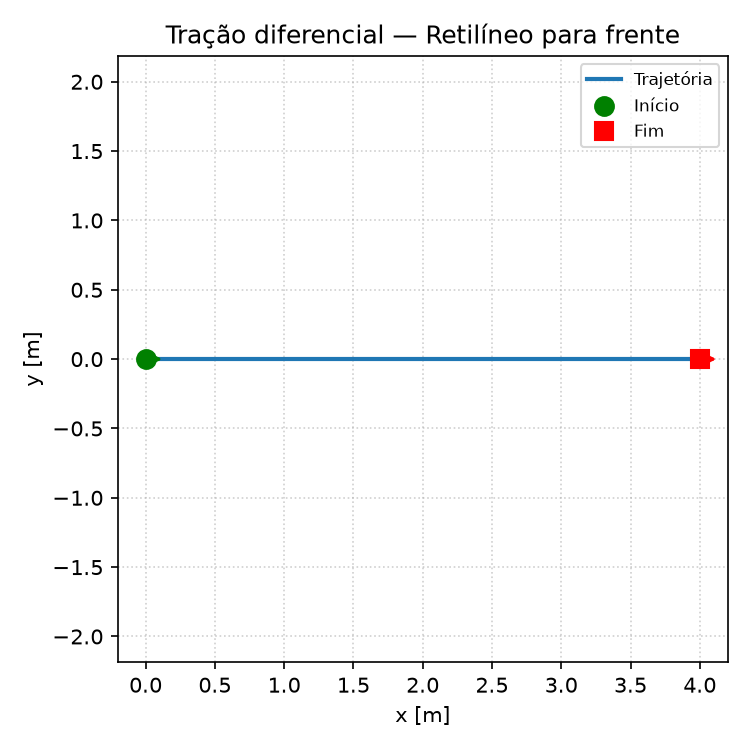
\includegraphics[width=\linewidth]{diffdrive_forward_traj.png}
    \caption{Frente}
  \end{subfigure}
  \begin{subfigure}{0.24\textwidth}
    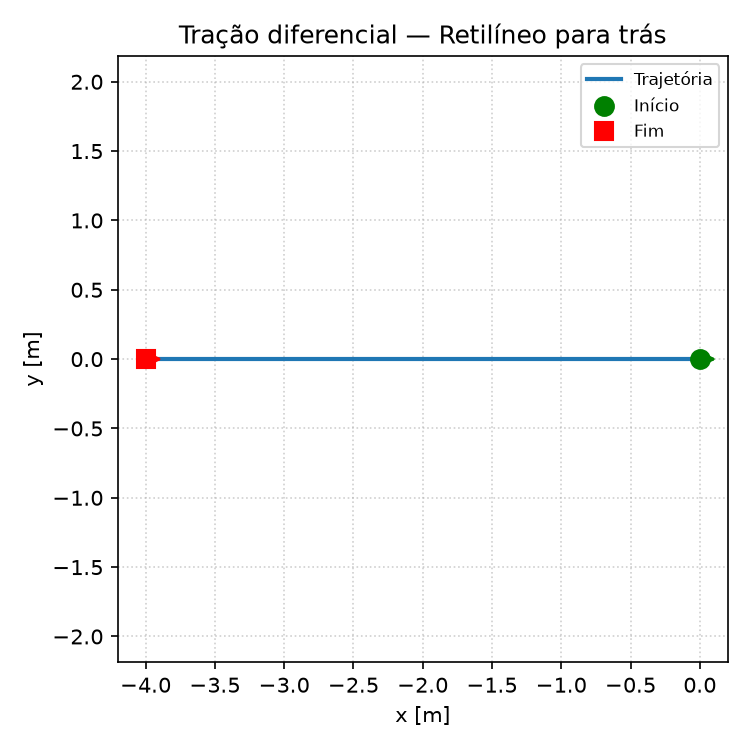
\includegraphics[width=\linewidth]{diffdrive_reverse_traj.png}
    \caption{Ré}
  \end{subfigure}
  \begin{subfigure}{0.24\textwidth}
    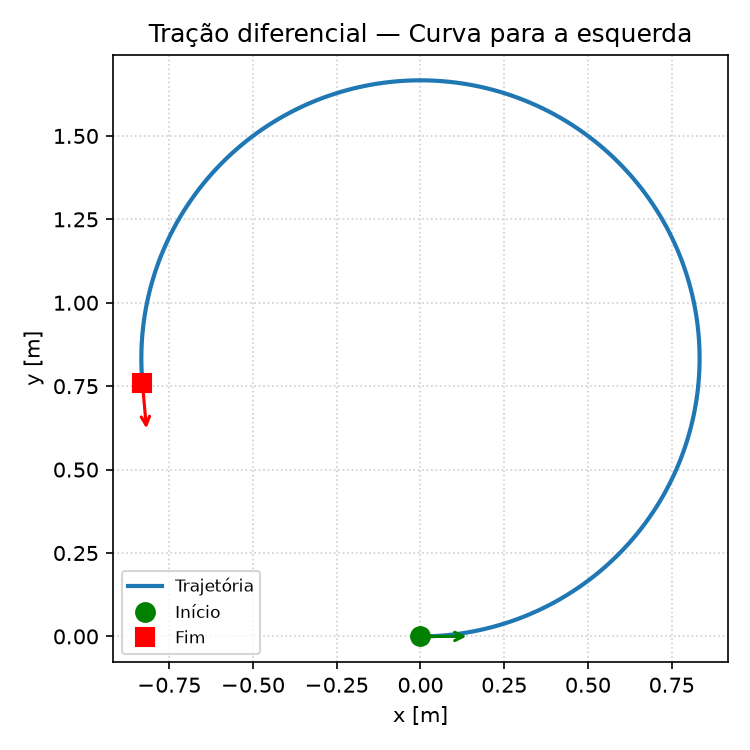
\includegraphics[width=\linewidth]{diffdrive_left_traj.png}
    \caption{Esquerda}
  \end{subfigure}
  \begin{subfigure}{0.24\textwidth}
    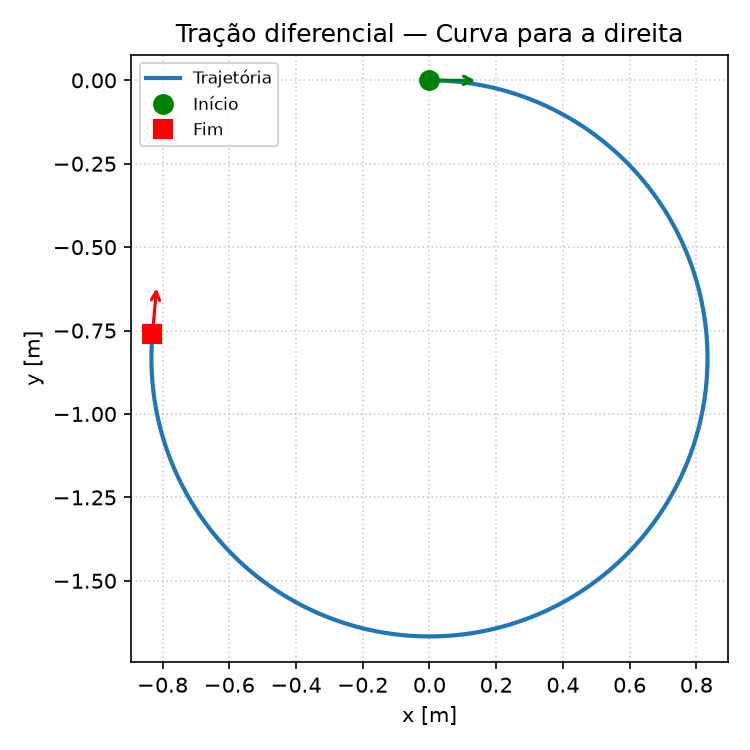
\includegraphics[width=\linewidth]{diffdrive_right_traj.png}
    \caption{Direita}
  \end{subfigure}
  \caption{Trajetórias $(X,Y)$ do robô de \textbf{tração diferencial}.}
  \label{fig:dd-traj}
\end{figure}

\begin{figure}[H]
  \centering
  \begin{subfigure}{0.24\textwidth}
    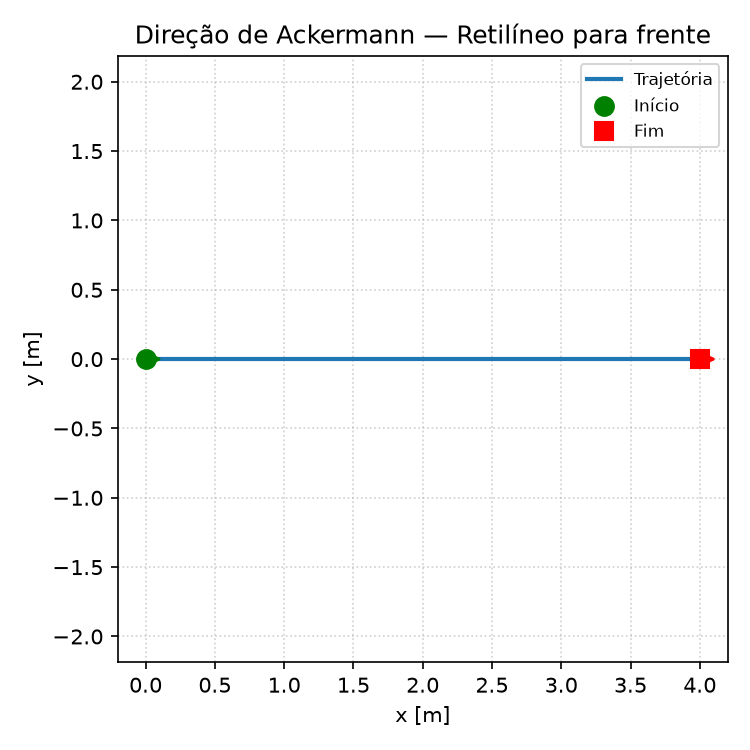
\includegraphics[width=\linewidth]{ackermann_forward_traj.png}
    \caption{Frente}
  \end{subfigure}
  \begin{subfigure}{0.24\textwidth}
    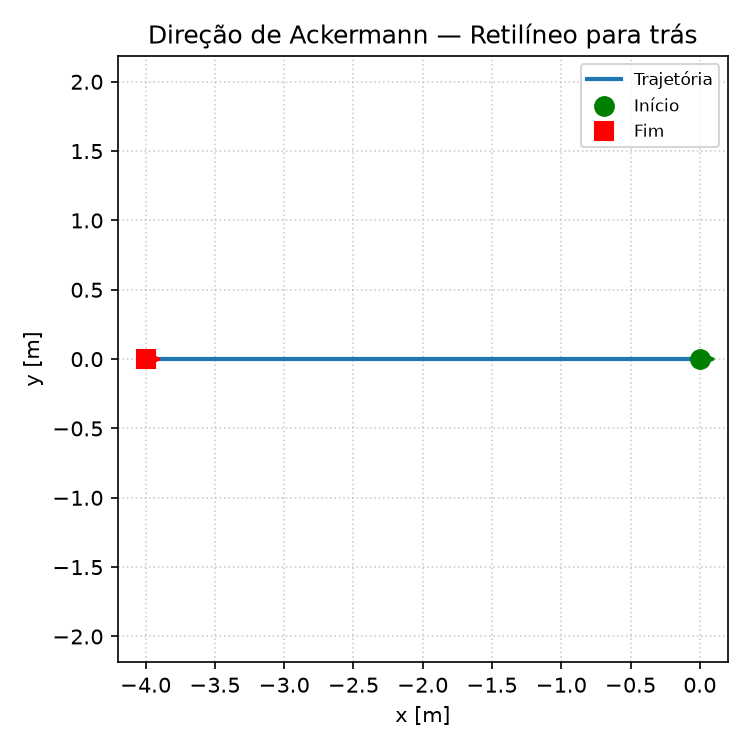
\includegraphics[width=\linewidth]{ackermann_reverse_traj.png}
    \caption{Ré}
  \end{subfigure}
  \begin{subfigure}{0.24\textwidth}
    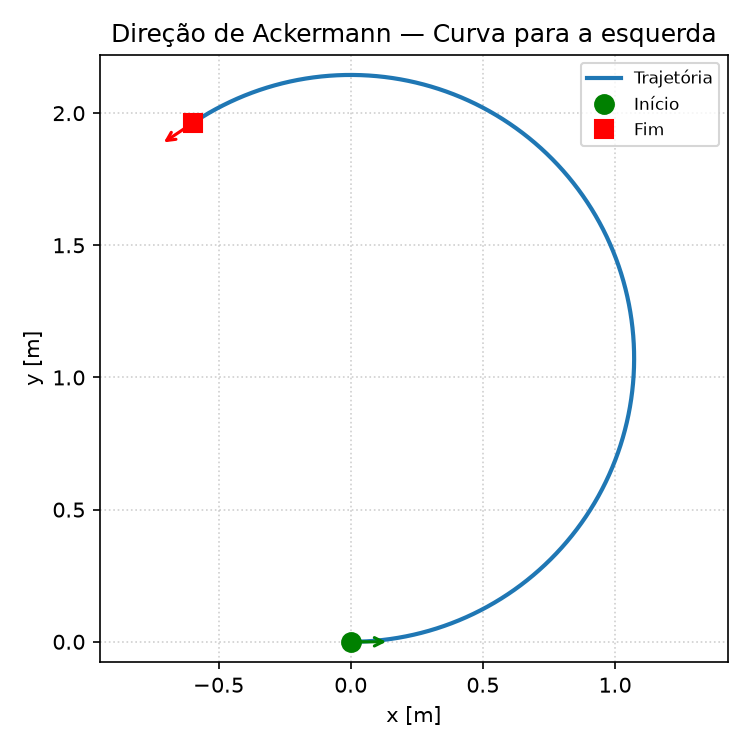
\includegraphics[width=\linewidth]{ackermann_left_traj.png}
    \caption{Esquerda}
  \end{subfigure}
  \begin{subfigure}{0.24\textwidth}
    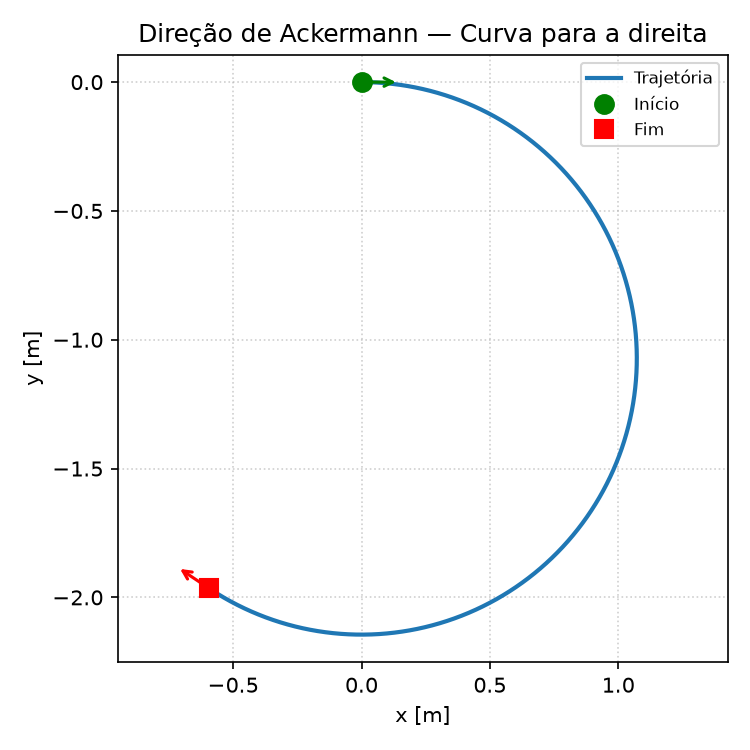
\includegraphics[width=\linewidth]{ackermann_right_traj.png}
    \caption{Direita}
  \end{subfigure}
  \caption{Trajetórias $(X,Y)$ do robô de \textbf{direção de Ackermann}.}
  \label{fig:ack-traj}
\end{figure}

\begin{figure}[H]
  \centering
  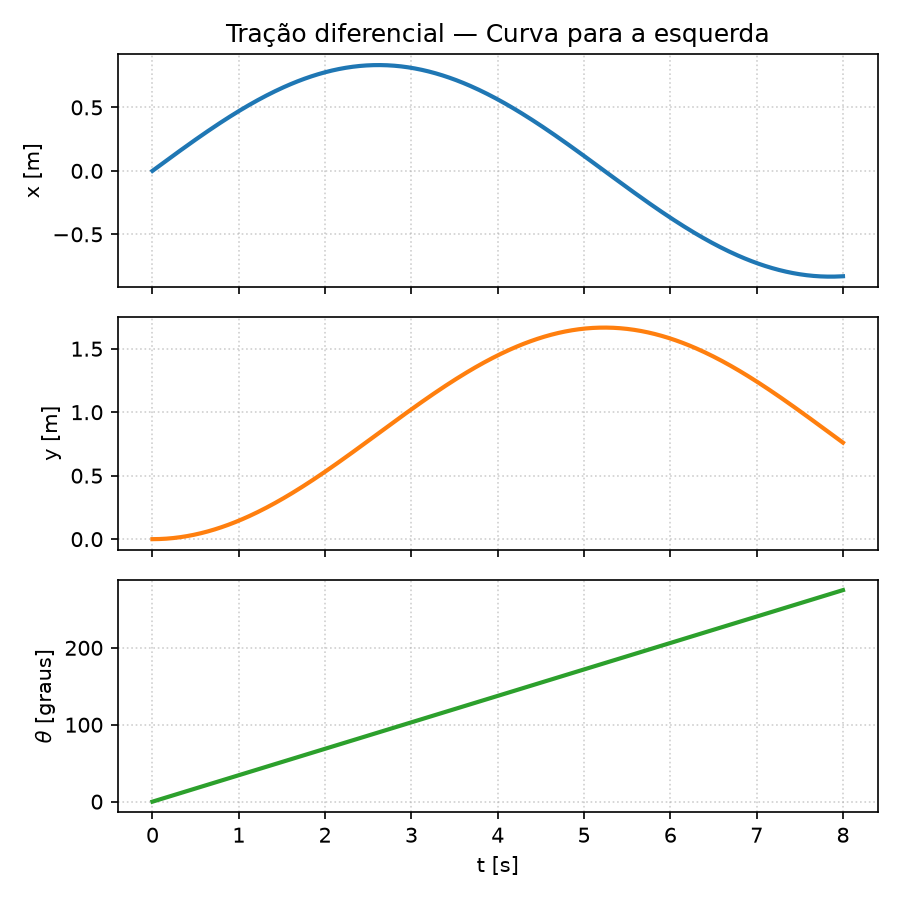
\includegraphics[width=0.55\linewidth]{diffdrive_left_states.png}
  \caption{Exemplo de evolução das variáveis de estado
  $x(t),\,y(t),\,\theta(t)$ (diferencial, curva à esquerda). Arquivos
  análogos são gerados para todos os cenários e ambos os robôs.}
  \label{fig:states}
\end{figure}

% ===========================================================================
\section{Simulação da Cinemática Direta via Integração Numérica}
% ===========================================================================

A cinemática direta integra o sistema de EDOs
$\dot{\mathbf{q}} = f(\mathbf{q},\mathbf{u})$ dado por~\eqref{eq:diffdrive}
ou~\eqref{eq:ackermann}, a partir de $\mathbf{q}(0)$ e de um sinal de
comando $\mathbf{u}(t)$. Como não há solução fechada geral para
$\theta(t)$ arbitrário, emprega-se integração numérica com passo
$\Delta t = \SI{0.02}{s}$ (\texttt{src/robotica/integrators.py}).

\paragraph{Integração de Euler (1ª ordem).}
\begin{equation}
  \mathbf{q}_{k+1} = \mathbf{q}_k + \Delta t\, f(\mathbf{q}_k,\mathbf{u}_k).
\end{equation}

\paragraph{Runge--Kutta de 4ª ordem (RK4).}
\begin{align}
  \mathbf{k}_1 &= f(\mathbf{q}_k,\mathbf{u}_k), &
  \mathbf{k}_2 &= f(\mathbf{q}_k + \tfrac{\Delta t}{2}\mathbf{k}_1,\mathbf{u}_k),\notag\\
  \mathbf{k}_3 &= f(\mathbf{q}_k + \tfrac{\Delta t}{2}\mathbf{k}_2,\mathbf{u}_k), &
  \mathbf{k}_4 &= f(\mathbf{q}_k + \Delta t\,\mathbf{k}_3,\mathbf{u}_k),\notag\\
  \mathbf{q}_{k+1} &= \mathbf{q}_k + \tfrac{\Delta t}{6}
    (\mathbf{k}_1 + 2\mathbf{k}_2 + 2\mathbf{k}_3 + \mathbf{k}_4). &&
\end{align}
O comando é mantido constante dentro de cada passo (segurador de ordem
zero). Adotou-se o RK4 como padrão por seu menor erro de truncamento
($O(\Delta t^4)$ contra $O(\Delta t)$ do Euler): em uma trajetória
circular de referência, o erro final de raio do RK4 é ordens de grandeza
menor que o do Euler para o mesmo $\Delta t$. O método é selecionável
por linha de comando (\texttt{--integrator euler|rk4}).

\paragraph{Validação.} Os casos-limite conferem com a solução analítica:
avanço reto ($x\approx vT$), giro puro ($\theta\approx\omega T$) e arco de
Ackermann de raio $R=L/\tan\phi$. As animações em
\texttt{outputs/animations/} ilustram o movimento contínuo de cada cenário.

\end{document}
